\documentclass[10pt]{article}
%DIF LATEXDIFF DIFFERENCE FILE
%DIF DEL old.tex    Sat Jul 16 21:14:46 2022
%DIF ADD main.tex   Sat Jul 16 21:44:32 2022
\usepackage[utf8]{inputenc}
\usepackage{geometry}
\usepackage[sort, numbers]{natbib}
\usepackage{pxfonts}
\usepackage{graphicx}
\usepackage{setspace}
\usepackage{hyperref}
\usepackage{lineno}
\usepackage{authblk}

\doublespacing
\linenumbers

\title{Fitness tracking reveals task-specific associations between
%DIF 16c16
%DIF <   memory, mental health, and exercise}
%DIF -------
  memory, mental health, and physical activity} %DIF > 
%DIF -------
\author[1, $\star$]{Jeremy R. Manning}
\author[1]{Gina M. Notaro}
\author[1]{Esme Chen}
\author[1]{Paxton C. Fitzpatrick}
\affil[1]{Dartmouth College, Hanover, NH}
\affil[$\star$]{Address correspondence to
  jeremy.r.manning@dartmouth.edu}


\newcommand{\devices}{S1}
\newcommand{\frDetail}{S2}
\newcommand{\natDetail}{S3}
\newcommand{\vocabDetail}{S4}
\newcommand{\spatialDetail}{S5}
\newcommand{\fitDists}{S6}
\newcommand{\fitDistgridImmediate}{S7}
\newcommand{\fitScatterImmediate}{S8}
\newcommand{\fitDistgridDelayed}{S9}
\newcommand{\fitScatterDelayed}{S10}
\newcommand{\behBehCorr}{S11}
\newcommand{\fitFitCorr}{S12}
\newcommand{\demDemCorr}{S13}
\newcommand{\allCorr}{S14}
\newcommand{\activityTimecourse}{S15}
\newcommand{\cardioTimecourse}{S16}
\newcommand{\sleepTimecourse}{S17}
\newcommand{\activityTimecourseMH}{S18}
\newcommand{\cardioTimecourseMH}{S19}
\newcommand{\sleepTimecourseMH}{S20}
%DIF PREAMBLE EXTENSION ADDED BY LATEXDIFF
%DIF UNDERLINE PREAMBLE %DIF PREAMBLE
\RequirePackage[normalem]{ulem} %DIF PREAMBLE
\RequirePackage{color}\definecolor{RED}{rgb}{1,0,0}\definecolor{BLUE}{rgb}{0,0,1} %DIF PREAMBLE
\providecommand{\DIFaddtex}[1]{{\protect\color{blue}\uwave{#1}}} %DIF PREAMBLE
\providecommand{\DIFdeltex}[1]{{\protect\color{red}\sout{#1}}}                      %DIF PREAMBLE
%DIF SAFE PREAMBLE %DIF PREAMBLE
\providecommand{\DIFaddbegin}{} %DIF PREAMBLE
\providecommand{\DIFaddend}{} %DIF PREAMBLE
\providecommand{\DIFdelbegin}{} %DIF PREAMBLE
\providecommand{\DIFdelend}{} %DIF PREAMBLE
\providecommand{\DIFmodbegin}{} %DIF PREAMBLE
\providecommand{\DIFmodend}{} %DIF PREAMBLE
%DIF FLOATSAFE PREAMBLE %DIF PREAMBLE
\providecommand{\DIFaddFL}[1]{\DIFadd{#1}} %DIF PREAMBLE
\providecommand{\DIFdelFL}[1]{\DIFdel{#1}} %DIF PREAMBLE
\providecommand{\DIFaddbeginFL}{} %DIF PREAMBLE
\providecommand{\DIFaddendFL}{} %DIF PREAMBLE
\providecommand{\DIFdelbeginFL}{} %DIF PREAMBLE
\providecommand{\DIFdelendFL}{} %DIF PREAMBLE
%DIF HYPERREF PREAMBLE %DIF PREAMBLE
\providecommand{\DIFadd}[1]{\texorpdfstring{\DIFaddtex{#1}}{#1}} %DIF PREAMBLE
\providecommand{\DIFdel}[1]{\texorpdfstring{\DIFdeltex{#1}}{}} %DIF PREAMBLE
\newcommand{\DIFscaledelfig}{0.5}
%DIF HIGHLIGHTGRAPHICS PREAMBLE %DIF PREAMBLE
\RequirePackage{settobox} %DIF PREAMBLE
\RequirePackage{letltxmacro} %DIF PREAMBLE
\newsavebox{\DIFdelgraphicsbox} %DIF PREAMBLE
\newlength{\DIFdelgraphicswidth} %DIF PREAMBLE
\newlength{\DIFdelgraphicsheight} %DIF PREAMBLE
% store original definition of \includegraphics %DIF PREAMBLE
\LetLtxMacro{\DIFOincludegraphics}{\includegraphics} %DIF PREAMBLE
\newcommand{\DIFaddincludegraphics}[2][]{{\color{blue}\fbox{\DIFOincludegraphics[#1]{#2}}}} %DIF PREAMBLE
\newcommand{\DIFdelincludegraphics}[2][]{% %DIF PREAMBLE
\sbox{\DIFdelgraphicsbox}{\DIFOincludegraphics[#1]{#2}}% %DIF PREAMBLE
\settoboxwidth{\DIFdelgraphicswidth}{\DIFdelgraphicsbox} %DIF PREAMBLE
\settoboxtotalheight{\DIFdelgraphicsheight}{\DIFdelgraphicsbox} %DIF PREAMBLE
\scalebox{\DIFscaledelfig}{% %DIF PREAMBLE
\parbox[b]{\DIFdelgraphicswidth}{\usebox{\DIFdelgraphicsbox}\\[-\baselineskip] \rule{\DIFdelgraphicswidth}{0em}}\llap{\resizebox{\DIFdelgraphicswidth}{\DIFdelgraphicsheight}{% %DIF PREAMBLE
\setlength{\unitlength}{\DIFdelgraphicswidth}% %DIF PREAMBLE
\begin{picture}(1,1)% %DIF PREAMBLE
\thicklines\linethickness{2pt} %DIF PREAMBLE
{\color[rgb]{1,0,0}\put(0,0){\framebox(1,1){}}}% %DIF PREAMBLE
{\color[rgb]{1,0,0}\put(0,0){\line( 1,1){1}}}% %DIF PREAMBLE
{\color[rgb]{1,0,0}\put(0,1){\line(1,-1){1}}}% %DIF PREAMBLE
\end{picture}% %DIF PREAMBLE
}\hspace*{3pt}}} %DIF PREAMBLE
} %DIF PREAMBLE
\LetLtxMacro{\DIFOaddbegin}{\DIFaddbegin} %DIF PREAMBLE
\LetLtxMacro{\DIFOaddend}{\DIFaddend} %DIF PREAMBLE
\LetLtxMacro{\DIFOdelbegin}{\DIFdelbegin} %DIF PREAMBLE
\LetLtxMacro{\DIFOdelend}{\DIFdelend} %DIF PREAMBLE
\DeclareRobustCommand{\DIFaddbegin}{\DIFOaddbegin \let\includegraphics\DIFaddincludegraphics} %DIF PREAMBLE
\DeclareRobustCommand{\DIFaddend}{\DIFOaddend \let\includegraphics\DIFOincludegraphics} %DIF PREAMBLE
\DeclareRobustCommand{\DIFdelbegin}{\DIFOdelbegin \let\includegraphics\DIFdelincludegraphics} %DIF PREAMBLE
\DeclareRobustCommand{\DIFdelend}{\DIFOaddend \let\includegraphics\DIFOincludegraphics} %DIF PREAMBLE
\LetLtxMacro{\DIFOaddbeginFL}{\DIFaddbeginFL} %DIF PREAMBLE
\LetLtxMacro{\DIFOaddendFL}{\DIFaddendFL} %DIF PREAMBLE
\LetLtxMacro{\DIFOdelbeginFL}{\DIFdelbeginFL} %DIF PREAMBLE
\LetLtxMacro{\DIFOdelendFL}{\DIFdelendFL} %DIF PREAMBLE
\DeclareRobustCommand{\DIFaddbeginFL}{\DIFOaddbeginFL \let\includegraphics\DIFaddincludegraphics} %DIF PREAMBLE
\DeclareRobustCommand{\DIFaddendFL}{\DIFOaddendFL \let\includegraphics\DIFOincludegraphics} %DIF PREAMBLE
\DeclareRobustCommand{\DIFdelbeginFL}{\DIFOdelbeginFL \let\includegraphics\DIFdelincludegraphics} %DIF PREAMBLE
\DeclareRobustCommand{\DIFdelendFL}{\DIFOaddendFL \let\includegraphics\DIFOincludegraphics} %DIF PREAMBLE
%DIF LISTINGS PREAMBLE %DIF PREAMBLE
\RequirePackage{listings} %DIF PREAMBLE
\RequirePackage{color} %DIF PREAMBLE
\lstdefinelanguage{DIFcode}{ %DIF PREAMBLE
%DIF DIFCODE_UNDERLINE %DIF PREAMBLE
  moredelim=[il][\color{red}\sout]{\%DIF\ <\ }, %DIF PREAMBLE
  moredelim=[il][\color{blue}\uwave]{\%DIF\ >\ } %DIF PREAMBLE
} %DIF PREAMBLE
\lstdefinestyle{DIFverbatimstyle}{ %DIF PREAMBLE
	language=DIFcode, %DIF PREAMBLE
	basicstyle=\ttfamily, %DIF PREAMBLE
	columns=fullflexible, %DIF PREAMBLE
	keepspaces=true %DIF PREAMBLE
} %DIF PREAMBLE
\lstnewenvironment{DIFverbatim}{\lstset{style=DIFverbatimstyle}}{} %DIF PREAMBLE
\lstnewenvironment{DIFverbatim*}{\lstset{style=DIFverbatimstyle,showspaces=true}}{} %DIF PREAMBLE
%DIF END PREAMBLE EXTENSION ADDED BY LATEXDIFF

\begin{document}
\maketitle

\newpage
\begin{abstract}
  Physical \DIFdelbegin \DIFdel{exercise }\DIFdelend \DIFaddbegin \DIFadd{activity }\DIFaddend can benefit both physical and mental well-being.
  Different forms of exercise (e.g., aerobic versus anaerobic; running
  versus walking, swimming, or yoga; high-intensity interval training
  versus endurance workouts; etc.) impact physical fitness in
  different ways.  For example, running may substantially impact leg
  and heart strength but only moderately impact arm strength. We
  hypothesized that the mental benefits of \DIFdelbegin \DIFdel{exercise }\DIFdelend \DIFaddbegin \DIFadd{physical activity }\DIFaddend might be similarly
  differentiated.  We focused specifically on how different \DIFdelbegin \DIFdel{forms of
  exercise }\DIFdelend \DIFaddbegin \DIFadd{intensities of
  physical activity }\DIFaddend might relate to different aspects of memory and mental
  health.  To test our hypothesis, we collected (in aggregate) roughly
  a century's worth of fitness data.  We then asked participants to
  fill out surveys asking them to self-report on different aspects of
  their mental health.  We also asked participants to engage in a
  battery of memory tasks that tested their short and long term
  episodic, semantic, and spatial memory performance.  We found that
  participants with similar \DIFdelbegin \DIFdel{exercise }\DIFdelend \DIFaddbegin \DIFadd{physical activity }\DIFaddend habits and fitness profiles
  tended to also exhibit similar mental health and task performance
  profiles.  These effects were task-specific in that different
  \DIFdelbegin \DIFdel{exercise }\DIFdelend \DIFaddbegin \DIFadd{physical activity }\DIFaddend patterns or fitness characteristics varied with different
  aspects of memory, on different tasks.  Taken together, these
  findings provide foundational work for designing \DIFdelbegin \DIFdel{exercise
  }\DIFdelend \DIFaddbegin \DIFadd{physical activity
  }\DIFaddend interventions that target specific components of cognitive performance
  and mental health by leveraging low-cost fitness tracking devices.
\end{abstract}

\section*{Introduction}
Engaging in physical activity (exercise) can improve physical fitness
by increasing muscle strength \citep{RogeEvan93, Lind79, CranEtal13,
  Knut07}, bone density~\citep{ChilEtal12, BassRams94, LaynNels99},
cardiovascular performance~\citep{MaioEtal00, PollEtal00}, lung
capacity~\citep[][although see \cite{RomaEtal16}]{LazoEtal16}, and
endurance~\citep{WilmKnut03}.  \DIFdelbegin \DIFdel{Exercise }\DIFdelend \DIFaddbegin \DIFadd{Physical activity }\DIFaddend can also improve mental
health~\DIFdelbegin \DIFdel{\mbox{%DIFAUXCMD
\citep{Ragl90, MikkEtal17, TaylEtal85, DeslEtal09, Call04,
  PaluSchw00, BassSuzu17} }\hspace{0pt}%DIFAUXCMD
}\DIFdelend \DIFaddbegin \DIFadd{\mbox{%DIFAUXCMD
\citep{Ragl90, MikkEtal17, TaylEtal85, DeslEtal09, Call04,
  PaluSchw00, BassSuzu17, MorrEtal18, GordEtal17, MorrEtal22, HerrEtal10} }\hspace{0pt}%DIFAUXCMD
}\DIFaddend and cognitive
performance~\citep{ChanEtal12b, BrisEtal02, EtniEtal06, BassSuzu17}.

The physical benefits of exercise can be explained by stress-responses
of the affected body tissues. For example, skeletal muscles that are
taxed during exercise exhibit stress responses~\citep{MortEtal09} that
can in turn affect their growth or atrophy~\citep{SchiEtal13}.  By
comparison, the benefits of \DIFdelbegin \DIFdel{exercise }\DIFdelend \DIFaddbegin \DIFadd{physical activity }\DIFaddend on mental health are less direct.
For example, one hypothesis is that \DIFdelbegin \DIFdel{exercise }\DIFdelend \DIFaddbegin \DIFadd{physical activity }\DIFaddend leads to specific
physiological changes, such as increased aminergic synaptic
transmission and endorphin release, which in turn act on
neurotransmitters in the brain~\citep{PaluSchw00}.  Speculatively, if
different \DIFdelbegin \DIFdel{exercise }\DIFdelend \DIFaddbegin \DIFadd{physical activity }\DIFaddend regimens lead to different neurophysiological
responses, one might be able to map out a spectrum of signalling and
transduction pathways that are impacted by a given type, duration, and
intensity of \DIFdelbegin \DIFdel{exercise }\DIFdelend \DIFaddbegin \DIFadd{physical activity }\DIFaddend in each brain region.  For example, prior work
has shown that \DIFdelbegin \DIFdel{exercise }\DIFdelend \DIFaddbegin \DIFadd{physical activity }\DIFaddend increases acetylcholine levels, starting in
the vicinity of the exercised muscles~\citep{ShoeEtal97}.
Acetylcholine is thought to play an important role in memory
formation~\citep[e.g., by modulating specific synaptic inputs from
entorhinal cortex to the hippocampus, albeit in
rodents;][]{PalaEtal21}.  Given the central role that these medial
temporal lobe structures play in memory, changes in acetylcholine
might lead to specific changes in memory formation and retrieval.

In the present study, we hypothesize that (a) different \DIFdelbegin \DIFdel{exercise
regimens }\DIFdelend \DIFaddbegin \DIFadd{intensities of physical activity }\DIFaddend will have different, quantifiable impacts on cognitive
performance and mental health, and that (b) these impacts will be
\DIFdelbegin \DIFdel{consistant }\DIFdelend \DIFaddbegin \DIFadd{consistent }\DIFaddend across individuals.  To this end, we collected a year of
real-world fitness tracking data from each of 113 participants.  We
then asked each participant to fill out a brief survey in which they
self-evaluated and self-reported several aspects of their mental
health.  Finally, we ran each participant through a battery of memory
tasks, which we used to evaluate their memory performance along
several dimensions.  We searched the data for potential associations
between memory, mental health, and \DIFdelbegin \DIFdel{exercise}\DIFdelend \DIFaddbegin \DIFadd{physical activity}\DIFaddend .

 \section*{Methods}

    We ran an online experiment using the Amazon Mechanical Turk (MTurk)
    platform~\citep{GureEtal16}.  We collected data about each participant's fitness and
    \DIFdelbegin \DIFdel{exercise }\DIFdelend \DIFaddbegin \DIFadd{physical activity }\DIFaddend habits, a variety of self-reported measures concerning their
    mental health, and about their performance on a battery of memory
    tasks.

    
    
\subsection*{Experiment}
\subsubsection*{Participants}
We recruited experimental participants by posting our experiment as a
Human Intelligence Task (HIT) on the MTurk platform.
We limited participation to MTurk Workers who had been
assigned a ``master worker'' designation on the platform, given to workers
who score highly across several metrics on a large number of HITs,
according to a proprietary algorithm managed by Amazon.  One \DIFdelbegin \DIFdel{criteria
}\DIFdelend \DIFaddbegin \DIFadd{criterion
}\DIFaddend embedded into the algorithm is a requirement that master
workers must maintain a HIT acceptance rate of at least 95\%.  We further
limited our participant pool to participants who self-reported that
they were fluent in English and regularly used a Fitbit fitness
tracker device.  A total of 160 workers accepted our HIT in order to
participate in our experiment.  Of these, we excluded all participants
who failed to log into their Fitbit account (giving us access to their
anonymized fitness tracking data), encountered technical issues (e.g.,
by accessing the HIT using an incompatible browser, device, or
operating system), or who ended their participation prematurely,
before completing the full study.  In all, 113 participants
contributed usable data to the study.

For their participation, workers received a base payment of \$5 per
hour (computed in 15 minute increments, rounded up to the nearest 15
minutes), plus an additional performance-based bonus of up to \$5.
Our recruitment procedure and study protocol were approved by
Dartmouth's Committee for the Protection of Human Subjects.  We
obtained informed consent using an online form administered to all
prospective participants prior to enrolling them in our study.  All
methods were performed in accordance with the relevant guidelines and
regulations.

\paragraph{Gender, age, and race.}
Of the 113 participants who contributed usable data, 77 reported their gender as female, 35 as
male, and 1 chose not to report their gender.  Participants ranged in
age from \DIFdelbegin \DIFdel{19--68 }\DIFdelend \DIFaddbegin \DIFadd{19 to 68 }\DIFaddend years old (25\textsuperscript{th} percentile: 28.25
years; 50\textsuperscript{th} percentile: 32 years;
75\textsuperscript{th} percentile: 38 years).  Participants reported
their race as White (90 participants), Black or African American (11
participants), Asian (7 participants), Other (4 participants), and
American Indian or Alaska Native (3 participants).  One participant
opted not to report their race.

\paragraph{Languages.}
All participants reported that they were fluent in either 1 and 2
languages (25\textsuperscript{th} percentile: 1;
50\textsuperscript{th} percentile: 1; 75\textsuperscript{th}
percentile: 1), and that they were ``familiar'' with between 1 and 11
languages (25\textsuperscript{th} percentile: 1;
50\textsuperscript{th} percentile: 2; 75\textsuperscript{th}
percentile: 3).

\paragraph{Reported medical conditions and medications.}
Participants reported having and/or taking medications pertaining to the following medical conditions: anxiety or
depression (4 participants), recent head injury (2 participants), high
blood pressure (1 participant), bipolar disorder (1 participant),
hypothyroidism (1 participant), and other unspecified conditions or medications (1
participant).  Participants reported their current and typical stress
levels on a Likert scale as very relaxed (-2), a little relaxed (-1),
neutral (0), a little stressed (1), or very stressed (2).  The
``current'' stress level reflected participants' stress at the time
they participated in the experiment.
Their responses
ranged from -2 to 2 (current stress: 25\textsuperscript{th} percentile: -2;
50\textsuperscript{th} percentile: -1; 75\textsuperscript{th}
percentile: 1; typical stress: 25\textsuperscript{th} percentile: 0;
50\textsuperscript{th} percentile: 1; 75\textsuperscript{th}
percentile: 1).  Participants also reported their current level of
alertness on a Likert scale as very sluggish (-2), a little sluggish
(-1), neutral (0), a little alert (1), or very alert (2).  Their
responses ranged from -2 to 2 (25\textsuperscript{th} percentile: 0;
50\textsuperscript{th} percentile: 1; 75\textsuperscript{th}
percentile: 2).  Nearly all (111 out of 113) participants reported
that they had normal color vision, and 15 participants reported
uncorrected visual impairments (including dyslexia and uncorrected
near- or far-sightedness).

\paragraph{Residence and level of education.}
Participants reported their residence
as being located in the suburbs (36 participants), a large city (30
participants), a small city (23 participants), rural (14
participants), or a small town (10 participants).  Participants
reported their level of education as follows: College graduate (42
participants), Master's degree (23 participants), Some college (21
participants), High school graduate (9 participants), Associate's
degree (8 participants), Other graduate or professional school (5
participants), Some graduate training (3 participants), or Doctorate
(2 participants).

\paragraph{Reported water and coffee intake.}
Participants reported the number of 8~oz cups of water and coffee they had
consumed prior to accepting the HIT.  Water consumption ranged from \DIFdelbegin \DIFdel{0--6 }\DIFdelend \DIFaddbegin \DIFadd{0 to 6 }\DIFaddend cups (25\textsuperscript{th} percentile: 1;
50\textsuperscript{th} percentile: 3; 75\textsuperscript{th}
percentile: 4).  Coffee consumption ranged from \DIFdelbegin \DIFdel{0--4 }\DIFdelend \DIFaddbegin \DIFadd{0 to 4 }\DIFaddend cups (25\textsuperscript{th} percentile: 0;
50\textsuperscript{th} percentile: 1; 75\textsuperscript{th}
percentile: 2).


\subsubsection*{Tasks}
Upon accepting the HIT posted on MTurk, each worker was
directed to read and fill out a screening and consent form, and to
share access to their anonymized Fitbit data via their Fitbit account.
After consenting to participate in our study and successfully sharing their Fitbit
data, participants filled out a survey and then engaged in a series of
memory tasks (Fig.~\ref{fig:tasks}).  All stimuli and code for running
the full MTurk experiment may be found
\href{https://github.com/ContextLab/brainfit-task}{\underline{here}}.

\begin{figure}[tp]
\centering
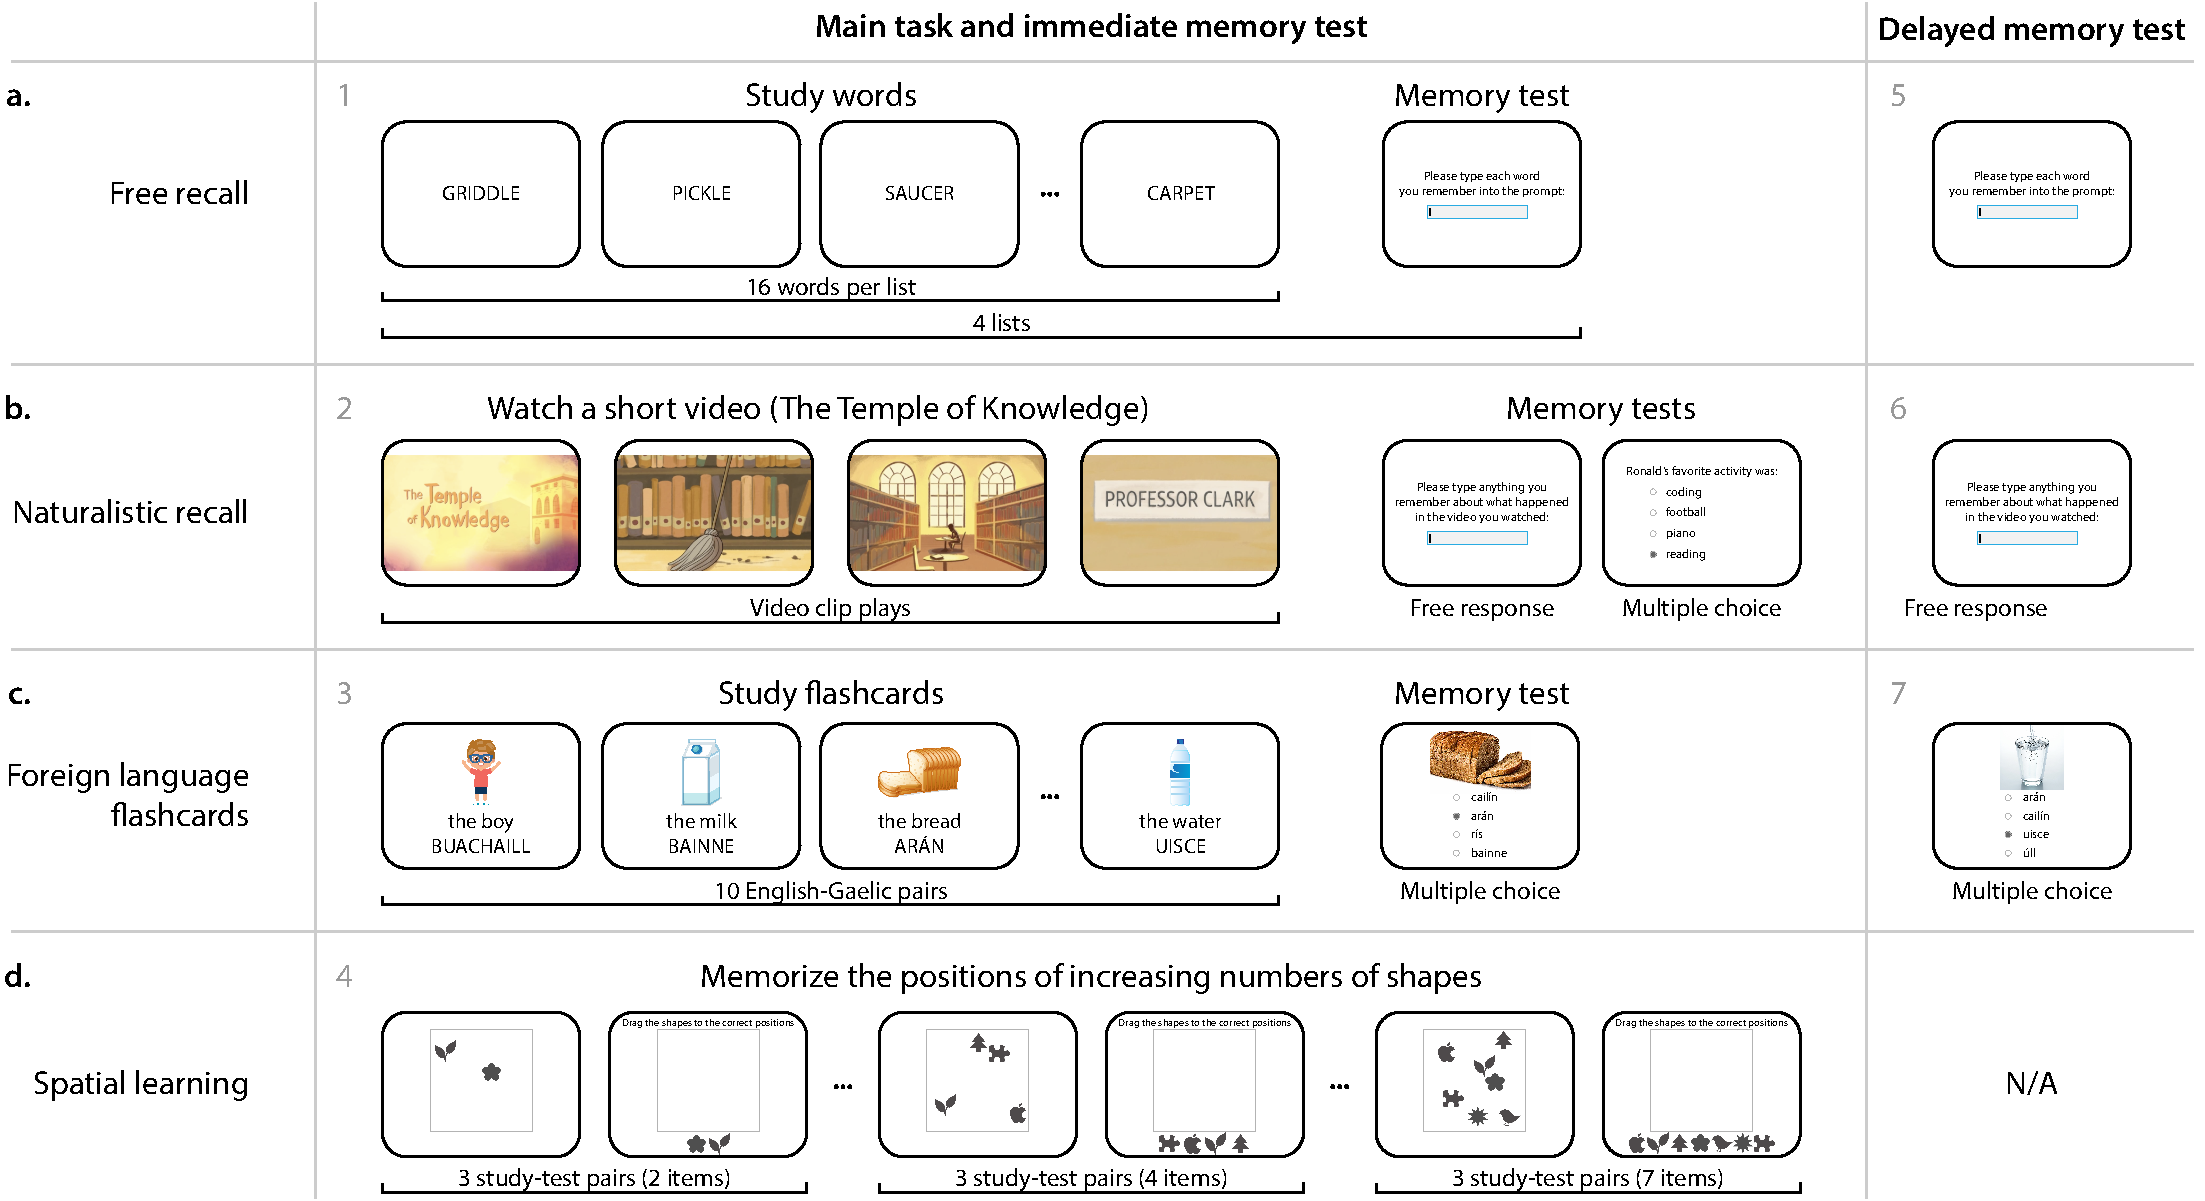
\includegraphics[width=1\textwidth]{figs/experiment}
\caption{\textbf{Battery of memory tasks.}  \textbf{a.  Free recall.}
Participants study 16 words (presented one at a time), followed by an
immediate memory test where they type
each word they remember from the just-studied list.  In the delayed
memory test, participants type any words they remember studying, from
any list.  \textbf{b. Naturalistic recall.}  Participants watch a
brief video, followed by two immediate memory tests.  The first test
asks participants to write out what happened in the video.  The second
test has participants answer a series of multiple choice questions
about the conceptual content of the video.  In the delayed memory
test, participants (again) write out what happened in the video.
\textbf{c. Foreign language flashcards.}  Participants study a
sequence of 10 English-Gaelic word pairs, each presented with an
illustration of the given word.  During an immediate memory test,
participants perform a multiple choice test where they select the
Gaelic word that corresponds to the given photograph.  During the
delayed memory test, participants perform a second multiple choice
test, where they select the Gaelic word that corresponds to each of a
new set of photographs.  \textbf{d. Spatial learning.}  In each trial,
participants
study a set of randomly positioned shapes.  Next, the shapes'
positions are altered, and participants are asked to drag the shapes
back to their previous positions.  \textbf{All panels.}  The gray
numbers denote the order in which participants experienced each task
or test.}
\label{fig:tasks}
\end{figure}

\paragraph*{Survey questions.}  We collected the following demographic
information from each participant: their birth year, gender, highest
(academic) degree achieved, race, language fluency, and language
familiarity.  We also collected information about participants'
health and wellness, including about their vision, alertness, stress, sleep, coffee
and water consumption, location of their residence, activity typically
required for their job, and \DIFdelbegin \DIFdel{exercise }\DIFdelend \DIFaddbegin \DIFadd{physical activity }\DIFaddend habits.


\paragraph*{Free recall (Fig.~\ref{fig:tasks}a).} 
Participants studied a sequence of four word lists, each comprising 16
words.  After studying each list, participants received an immediate
memory test, whereby they were asked to type (one word at a time) any
words they remembered from the just-studied list, in any order.

Words were presented for 2~s each, in black text on a white
background, followed by a 2~s blank (white) screen.  After the final
2~s pause, participants were given 90~s to type in as many words as
they could remember, in any order.  The memory test was constructed
such that the participant could only see the text of the current word
they were typing; when they pressed any non-letter key, the current
word was submitted and the text box they were typing in was cleared.
This was intended to prevent participants from retroactively editing
their previous responses.

The word lists participants studied were drawn from the categorized
lists reported by \cite{ZimaEtal18}.  Each participant was assigned
four unique randomly chosen lists (in a randomized order), selected
from a full set of 16 lists.  Each chosen list was then randomly
shuffled before presenting the words to the participants.
Participants also performed a final delayed memory test where they
were given 180~s to type out any words they remembered from
\textit{any} of the 4 lists they had studied.

Recalled words within an edit distance of 2 (i.e., a Levenshtein Distance less
than or equal to 2) of any word in the wordpool were ``autocorrected''
to their nearest match.  We also manually corrected clear typos or
misspellings by hand (e.g., we corrected ``hippoptumas'' to
``hippopotamus'', ``zucinni'' to ``zucchini'', and so on).  Finally,
we lemmatized each submitted word to match the plurality of the
matching wordpool word (e.g., ``bongo'' was corrected to ``bongos'',
and so on).  After applying these corrections, any submitted words
that matched words presented on the just-studied list were tagged as
``correct'' recalls, and any non-matching words were discarded as
``errors.''  Because participants were not allowed to edit the text
they entered, we chose not to analyze these putative ``errors,'' since
we could not distinguish typos from true misrememberings.

\paragraph*{Naturalistic recall (Fig.~\ref{fig:tasks}b).}
Participants watched a 2.5\DIFdelbegin \DIFdel{~minute }\DIFdelend \DIFaddbegin \DIFadd{-minute }\DIFaddend video clip entitled ``The Temple of
Knowledge.''  The video comprises an animated story told to StoryCorps
by Ronald Clark, who was interviewed by his daughter, Jamilah Clark.
The narrator (Ronald) discusses growing up living in an apartment over
the Washington Heights branch of the New York Public Library, where his
father worked as a custodian during the 1940s.

After watching the video clip, participants were asked to type out
anything they remembered about what happened in the video.  They typed
their responses into a text box, one sentence at a time.  When the
participant pressed the return key or typed any final punctuation mark
(``.'', ``!'', or ``?'') the text currently entered into the box was
``submitted'' and added to their transcript, and the text box was
cleared to prevent further editing of any already-submitted text.
This was intended to prevent participants from retroactively editing
their previous responses.  Participants were given up to 10~minutes to
enter their responses.  After 4~minutes, participants were given the
option of ending the response period early, e.g., if they felt they
had finished entering all \DIFdelbegin \DIFdel{of }\DIFdelend the information they remembered.  Each
participant's transcript was constructed from their submitted
responses by combining the sentences into a single document and
removing extraneous whitespace characters.  Following this \DIFdelbegin \DIFdel{4--10
minute }\DIFdelend \DIFaddbegin \DIFadd{4--10-minute }\DIFaddend free response period, participants were given a series of 10
multiple choice questions about the conceptual content of the story.
All participants received the same questions, in the same order.
Participants also performed a final delayed memory test, where they
carried out the free response recall task a second time, near the end
of the testing session.  This resulted in a second transcript, for
each participant.

\paragraph*{Foreign language flashcards (Fig.~\ref{fig:tasks}c).}
Participants studied a series of 10 English-Gaelic word pairs in a
randomized order.  We selected the Gaelic language both for its
relatively small number of native speakers and for its dissimilarity
to other commonly spoken languages amongst MTurk workers.
We verified (via self report) that all of our participants were fluent
in English and that they were neither fluent nor familiar with Gaelic.

Each word's ``flashcard'' comprised a cartoon depicting the given
word, the English word or phrase in lowercase text (e.g., ``the
boy''), and the Gaelic word or phrase in uppercase text (e.g.,
``BUACHAILL'').  Each flashcard was displayed for 4~s, followed by a
3~s interval (during which the screen was cleared) prior to the next
flashcard presentation.

After studying all 10 flashcards, participants were given a multiple
choice memory test where they were shown a series of novel
photographs, each depicting one of the 10 words they had learned.
They were asked to select which (of 4 unique options) Gaelic word went
with the given picture.  The 3 incorrect options were selected at
random (with replacement across trials), and the order in which the
choices appeared to the participant were also randomized.  Each of the
10 words they had learned were tested exactly once.

Participants also performed a final delayed memory test, where they
were given a second set of 10 questions (again, one per word they had
studied).  For this second set of questions participants were prompted
with a new set of novel photographs, and new randomly chosen incorrect
choices for each question.  Each of the 10 original words they had
learned were (again) tested exactly once during this final memory
test.



\paragraph*{Spatial learning (Fig.~\ref{fig:tasks}d).}
Participants performed a series of study-test trials where they
memorized the onscreen spatial locations of two or more shapes.
During the study phrase of each trial, a set of shapes appeared on the
screen for 10~s, followed by 2~s of blank (white) screen.  During the
test phase of each trial, the same shapes appeared onscreen again, but
this time they were vertically aligned and sorted horizontally in a
random order.  Participants were instructed to drag (using the mouse)
each shape to its studied position, and then to click a button to
indicate that the placements were complete.

In different study-test trials, participants learned the locations of
different numbers of shapes (always drawn from the same pool of 7
unique shapes, where each shape appeared at most one time per trial).
They first performed three trials where they learned the locations of
2 shapes; next three trials where they learned the locations of 3
shapes; and so on until their last three trials, where (during each
trial) they learned the locations of 7 shapes.  All told, each
participant performed 18 study-test trials of this spatial learning
task (3 trials for each of 2, 3, 4, 5, 6, and 7 shapes).


\subsubsection*{Fitness tracking using Fitbit devices}
To gain access to our study, participants provided us with access to
all data associated with their Fitbit account from the year (365
calendar days) up to and including the day they accepted the HIT.  We
filtered out all identifiable information (e.g., participant names,
GPS coordinates, etc.) prior to importing their data.

\subsubsection*{Collecting and processing Fitbit data}

The fitness tracking data associated with participants' Fitbit
accounts varied in scope and duration according to which device the
participant owned (Fig.~\devices), how often the participant wore
(and/or synced) their tracking device, and how long they had owned
their device.  For example, while all participants' devices supported
basic activity metrics such as daily step counts, only a subset of the
devices with heart rate monitoring capabilities provided information
about workout intensity, resting heart rate, and other related
measures.  Across all devices, we collected the following information:
heart rate data, sleep tracking data, logged bodyweight measurements,
logged nutrition measurements, Fitbit account and device settings, and
activity metrics.

\paragraph{Heart rate.}  If available, we extracted all heart rate
data collected by participants' Fitbit device(s) and associated with
their Fitbit profile.  Depending on the specific device model(s) and
settings, this included second-by-second, minute-by-minute, daily
summary, weekly summary, and/or monthly summary heart rate
information.  These summaries include information about participants'
average heart rates, and the amount of time they were estimated to
have spent in different ``heart rate zones'' (rest, out-of-range, fat
burn, cardio, or peak, as defined by their Fitbit profile), as well as
an estimate of the number of estimated calories burned while in each
heart rate zone.

\paragraph{Sleep.}  If available, we extracted all sleep data
collected by participants' Fitbit device(s).  Depending on the
specific device model(s) and settings, this included nightly estimates
of the duration and quality of sleep, as well as the amount of time
spent in each sleep stage (awake, REM, light, or deep).

\paragraph{Weight.}  If available, we extracted any weight-related
information affiliated with participants' Fitbit accounts within 1
year prior to enrolling in our study.  Depending on their specific
device model(s) and settings, this included their weight, body mass
index, and/or body fat percentage.

\paragraph{Nutrition.} If available, we extracted any
nutrition-related information affiliated with participants' Fitbit
accounts within 1 year prior to enrolling in our study. Depending on
their specific account settings and usage behaviors, this included a
log of the specific foods they had eaten (and logged) over the past
year, and the amount of water consumed (and logged) each day.

\paragraph{Account and device settings.}  We extracted any settings
associated with participants' Fitbit accounts to determine (a) which
device(s) and model(s) are associated with their Fitbit account, (b)
time(s) when their device(s) were last synced, and (c) battery
level(s).

\paragraph{Activity metrics.}  If available, we extracted any
activity-related information affiliated with participants' Fitbit
accounts within 1 year prior to enrolling in our study.  Depending on
their specific device model(s) and settings, this included: daily step
counts; daily amount of time spent in each activity level (sedentary,
lightly active, fairly active, or very active, as defined by their
account settings and preferences); daily number of floors climbed;
daily elevation change; and daily total distance traveled.



\subsubsection*{Comparing recent versus baseline measurements.}
We were interested in separating out potential associations between
\textit{absolute} fitness metrics and \textit{relative} metrics.  To
this end, in addition to assessing potential raw (absolute) fitness
metrics, we also defined a simple measure of recent changes in those
metrics, relative to a baseline:
\[
  \Delta_{R, B} m = \frac{B \sum_{i = 1}^R
  m(i)}{R \sum_{i=R + 1}^{R+B}m(i)},
\]
where $m(i)$ is the value of metric $m$ from $i - 1$ days prior to
testing (e.g., $m(1)$ represents the value of $m$ on the day the
participant accepted the HIT, and $m(10)$ represents the value of $m$
9 days prior to accepting the HIT\DIFaddbegin \DIFadd{)}\DIFaddend .  We set $R = 7$ and $B = 30$.  In
other words, to estimate recent changes in any metric $m$, we divided
the average value of $m$ taken over the prior week by the average
value of $m$ taken over the 30 days before that.


\subsubsection*{Exploratory correlation analyses}
We used a bootstrap procedure to identify reliable correlations
between different memory-related, fitness-related, and
demographic-related variables.  For each of $N = 10,000$ iterations, we
selected (with replacement) a sample of 113 participants to include.
This yielded, for each iteration, a sampled ``data matrix'' with one
row per sampled participant and one column for each measured variable.
When participants were sampled multiple times in a given iteration, as
was often the case, this matrix contained duplicate rows.  Next, we computed the Pearson's correlation
between each pair of columns.  This yielded, for each pair of columns,
a distribution of $N$ bootstrapped correlation coefficients.  If
$97.5\%$ or fewer of the coefficients for a given pair of columns had the
same sign, we excluded the pair from further analysis and considered
the expected correlation between those columns to be undefined.  If
$> 97.5\%$ of the coefficients for a given pair of columns had the
same sign (corresponding to a bootstrap-estimated two-tailed $p$
threshold of 0.05), we computed the expected correlation coefficient as:
\[
  \mathbb{E}_{i, j}\left[ r\right] = \tanh\left(\frac{1}{N} \sum_{n=1}^N
  \tanh^{-1}(\mathrm{corr}\left(m(i)_n, m(j)_n\right))\right),
\]
where $m(x)_n$ represents column $x$ of the bootstrapped data matrix
for iteration $n$, $\tanh$ is the hyperbolic tangent, and $\tanh^{-1}$
is the inverse hyperbolic tangent.  We estimated the corresponding $p$-values
for these correlations as one minus the proportion of bootstrapped
correlations with the same sign, multiplied by two.

\subsubsection*{Reverse correlation analyses}
We sought to characterize potential associations between the \textit{dynamics}
of participants' fitness-related activities leading up to the time
they participated in a memory task and their performance on the given
task.  For each fitness-related variable, we constructed a timeseries
matrix whose rows corresponded to timepoints (sampled once per day)
leading up to the day the participant accepted the HIT for our study,
and whose columns corresponded to different participants.  These
matrices often contained missing entries, since different
participants' Fitbit devices tracked fitness-related activities
differently.  For example, participants whose Fitbit devices lacked
heart rate sensors would have missing entries for any heart
rate-related variables.  Or, if a given participant neglected to wear
their fitness tracker on a particular day, the column corresponding to
that participant would have missing entries for that day.  To create
stable estimates, we smoothed the timeseries of each fitness measure
using a sliding window of 1 week.  In other words, for each fitness
measure, we replaced the ``observed
value'' for each day with the average values of that measure (when
available) over the \DIFdelbegin \DIFdel{7 day }\DIFdelend \DIFaddbegin \DIFadd{7-day }\DIFaddend interval ending on the given day.

In addition to this set of matrices storing timeseries data for each
fitness-related variable, we also constructed a memory performance
matrix, $M$, whose rows corresponded to different memory-related
variables, and whose columns corresponded to different participants.
For example, one row of the memory performance matrix reflected the
average proportion of words (across lists) that each participant
remembered during the immediate free recall test, and so on.

Given a fitness timeseries matrix, $F$, we computed the weighted
average and weighted standard error of the mean of each row of $F$,
where the weights were given by a particular memory-related variable
(row of $M$).  For example, if $F$ contained participants' daily step
counts, we could use any row of $M$ to compute a weighted average
across any participants who contributed step count data on each day.
Choosing a row of $M$ that corresponded to participants' performance
on the naturalistic recall task would mean that participants who
performed better on the naturalistic recall task would contribute more
to the weighted average timeseries of daily step counts.
Specifically, for each row, $t$, of $F$, we computed the weighted
average (across the $S$ participants) as:
\[
\bar{f}(t) = \sum_{s=1}^S \dot{m}(s) F(t, s),
\]
where $\dot{m}$ denotes the normalized min-max scaling of $m$ (the row
of $M$ corresponding to the chosen memory-related variable):
\[
  \dot{m} = \frac{m}{\sum_{s=1}^S \hat{m}(s)},
\]
where
\[
  \hat{m} = (1 - \epsilon)\frac{m - \min(m)}{\max(m) - \min(m)} + \epsilon.
\]
Here, $\epsilon$ provides a lower bound on the influence of the
lowest-weighted participant's data.  We defined $\epsilon = 0.001$,
ensuring that the lowest-weighted participant had relatively low (but
non-zero) influence.  We computed the weighted standard error of the
mean as:
\[
\mathrm{SEM}_m\left(f(t)\right) = \frac{\left| \sum_{s=1}^S \left( F(t, s) -
    \bar{f}(t)\right) \right|}{\sqrt{S}}.
\]
When a given row of $F$ was missing data from one or more
participants, those participants were excluded from the weighted
average for the corresponding timepoint and the weights (across all
remaining participants) were re-normalized to sum to 1.  The above
procedure yielded, for each memory variable, a timeseries of weighted
average (and weighted standard error of the mean) fitness tracking
values leading up to the day of the experiment.

\section*{Results}
Before testing our main hypotheses, we examined the behavioral data
from each of four memory tasks: a random word list learning ``free
recall'' task (Fig.~\ref{fig:tasks}); a naturalistic recall task whereby participants watched
a short video and then recounted the narrative; a foreign language
``flashcards'' task; and a spatial learning task.  Each of the first
three tasks (free recall, naturalistic recall, and the flashcards
task) included both an immediate (short term) memory test and a
delayed (long term) memory test.  The spatial learning task included
only an immediate test. Participants in all four tasks exhibited
general trends and tendencies that have been previously reported in
prior work.  We were also interested in characterizing the variability
in task performance across participants.  For example, if all
participants exhibited near-identical behaviors or performance on a
given task, we would be unable to identify how memory performance on
that task varied with mental health or \DIFdelbegin \DIFdel{exercise}\DIFdelend \DIFaddbegin \DIFadd{physical activity}\DIFaddend .

When participants engaged in free recall of random word lists, they
displayed strong primacy and recency effects~\citep{Murd62a} on the
immediate memory tests (as reflected by improved memory for early and
late list items; Fig.~\ref{fig:immediate_behavior}a, left and right
panels).  On the delayed memory test, the recency effect was
substantially diminished (Fig.~\ref{fig:delayed_behavior}a, left and
right panels), consistent with myriad previous studies~\citep[for
review see][]{Kaha12}.  Participants also tended to cluster their
recalls according to the words' study positions~\citep{Kaha96} on both
the immediate (Fig.~\ref{fig:immediate_behavior}a, middle panel) and
delayed (Fig.~\ref{fig:delayed_behavior}a, middle panel) memory tests.

When participants engaged in naturalistic recall by recounting the
narrative of a short story video, they reliably and accurately
remembered the major narrative events on both the immediate
(Fig.~\ref{fig:immediate_behavior}b) and delayed
(Fig.~\ref{fig:delayed_behavior}b) tests.  This is consistent with
prior work showing that memory for rich narratives is both detailed
and accurate~\citep{HeusEtal21, ChenEtal17}.

Performance on the foreign language flashcards task (immediate:
Fig.~\ref{fig:immediate_behavior}c; delayed:
Fig.~\ref{fig:delayed_behavior}c) varied substantially across
participants, and did not show any clear serial position effects.
Participants also displayed substantial variation in performance on
the spatial learning task (Fig.~\ref{fig:immediate_behavior}d).  In
general, participants reported the shape's positions more accurately
when there were fewer shapes.  However, both the baseline estimation accuracy and
the rate of decrease in accuracy as a function of increasing number of
memorized locations varied substantially across participants.

\begin{figure}[tp]
\centering
\includegraphics[width=1\textwidth]{figs/behavior_overview_immediate}
\caption{\textbf{Immediate memory tests.}  \textbf{a. Free recall.}
  Left: probability of recalling each word first as a function of its
  presentation position.  Middle: probability of transitioning between
successively recalling the word presented at position $i$, followed by
word presented at position $i + \mathrm{Lag}$.  Right: probability of
recalling each word as a function of its presentation position.  See
Figure~\frDetail~for additional details.
\textbf{b. Naturalistic recall.}  Top: 2D embedding of a 2.5\DIFdelbeginFL \DIFdelFL{~min }\DIFdelendFL \DIFaddbeginFL \DIFaddFL{-min }\DIFaddendFL video
clip; each dot reflects a narrative event (red denotes early events
and blue denotes later events).  Bottom: 2D embedding of the averaged
transcripts of participants' recountings of the narrative (dots: same
format as top panel).  The arrows denote the average trajectory
directions through the corresponding region of text embedding space,
for any participants whose recountings passed through that region.
Blue arrows denote statistically reliable agreement across
participants ($p < 0.05$, corrected).  See Figure~\natDetail~for
additional details.  \textbf{c. Foreign language
  flashcards.} Each bar denotes the average proportion of correctly
recalled Gaelic-English word pairs from early (first 3), late (last
3), or all (i.e., all 10) study positions.  See
Figure~\vocabDetail~for additional details.  \textbf{d. Spatial
  learning.}  Average estimation error in shape locations as a
function of the number of shapes.  See Figure~\spatialDetail~for
additional details.  All panels: error bars and error
ribbons denote bootstrap-estimated 95\% confidence intervals.  Shading
(saturation) denotes results for different subsets of participants
assigned based on their task performance (Figs.~\frDetail,
\natDetail, \vocabDetail, and \spatialDetail~provide information about
which performance metrics and values the shading reflects; in general
more saturated colors denote participants who performed better on the
given task.)  In Panel d, participants are grouped in two ways; in the
left panel, participants are grouped according to the $y$-intercepts of regression lines (estimation error as a
function of the number of shapes); in the right panel, participants
are grouped according to the slopes of the same regression lines.}
\label{fig:immediate_behavior}
\end{figure}

\begin{figure}[tp]
\centering
\includegraphics[width=1\textwidth]{figs/behavior_overview_delayed}
\caption{\textbf{Delayed memory tests.}  \textbf{a.  Free recall.}
  These panels are in the same format as
  Figure~\ref{fig:immediate_behavior}a, but they reflect performance
  on the delayed free recall task.  For additional details see
  Figure~\frDetail.  \textbf{b. Naturalistic recall.}  These panels
  are in the same format as Figure~\ref{fig:immediate_behavior}b, but
  the right panel reflects performance on the delayed naturalistic
  recall task.  For additional details see Figure~\natDetail.
  \textbf{c. Foreign language flashcards.} This panel is in the same
  format as Figure~\ref{fig:immediate_behavior}c, but it reflects
  performance on the delayed flashcards test.  For additional details
  see Figure~\vocabDetail.}
\label{fig:delayed_behavior}
\end{figure}

In addition to observing substantial across-participant variability in
memory performance, we also observed substantial variability in
participants' fitness and activity metrics
(Fig.~\ref{fig:fitness_summary}).  We examined recent measurements,
averaged over the week prior to testing
(Fig.~\ref{fig:fitness_summary}a), baselined measurements (average
over the prior week, divided by the average over the preceding 30 days;
Fig.~\ref{fig:fitness_summary}b), along with more gradually varying
measures that tended to remain relatively static over timescales of
weeks to months (Fig.~\ref{fig:fitness_summary}c).
Figure~\fitDists~displays across-participant
distributions for a broad selection of these measures, and Figures~\fitDistgridImmediate,
\fitScatterImmediate, \fitDistgridDelayed, and \fitScatterDelayed~show
different participants' fitness metrics, broken down by their
performance on different memory tasks.

\begin{figure}[tp]
\centering
\includegraphics[width=0.8\textwidth]{figs/fitness_distributions_summary}
\caption{\textbf{Fitness measures.}  \textbf{a. Recent measures.}
  Resting heart rate (HR) and daily step counts, averaged over the
  week prior to testing.  \textbf{Baseline-normalized measures.}
  Resting heart rate and daily step counts averaged over the week
  prior to testing, divided by the average resting heart rate and step
counts averaged over the preceding month.  \textbf{Static measures.}
Body mass index (BMI), body fat percentage, and weight (in kg).  For
more information see Figures~\fitDists, \fitDistgridImmediate,
\fitScatterImmediate, \fitDistgridDelayed, and \fitScatterDelayed.}
\label{fig:fitness_summary}
\end{figure}

We wondered about potential links between the different aspects of
participants' data.  For example, if people who \DIFdelbegin \DIFdel{exercised in a
particular way }\DIFdelend \DIFaddbegin \DIFadd{engaged in particular intensities of physical activity }\DIFaddend also tended to perform better on a given memory task,
this could suggest that either (a) some property intrinsic to
participants who exercised in a particular way might also affect their
memory performance on the given task, and/or (b) particular \DIFdelbegin \DIFdel{exercise
}\DIFdelend \DIFaddbegin \DIFadd{physical activity
}\DIFaddend behaviors could have a causal impact on memory performance.  We
carried out an exploratory analysis whereby we used a bootstrap-based
approach to identify reliable correlations between different aspects
of memory performance (Fig.~\behBehCorr), different aspects of fitness
(Fig.~\fitFitCorr), different demographic attributes
(Fig.~\demDemCorr), and correlations between memory performance,
fitness information, and demographic attributes (Fig.~\allCorr).
Specifically, we sought to identify correlations that were present in
the same direction (i.e., positive or negative) across different
subsets of participants.  For each test, we report the average correlation (taken
across 10,000 subsets of participants, chosen with replacement) and
an associated two-tailed $p$-value, estimated as
\[
p = 2 \times (1 - q),
\]
where $q$ is the proportion of those
10,000 subsets that exhibited correlations in the same direction  (see
\textit{Exploratory correlation analyses}).  When all 10,000 randomly
chosen subsets of participants exhibited correlations in the same
direction (i.e., all positive correlations or all negative
correlations), we report the $p$-value as $p < 0.0001$.

Several patterns emerged from these analyses.  First, we found that
participants' performance on the (within-task) immediate versus delayed memory tests
from the free recall, naturalistic recall, and foreign language
flashcards tasks were positively correlated ($r$s $> 0.25$, $p$s $< 0.003$).  This suggests that, within each of these tasks,
similar processes or constraints may influence both short term and
long term information retrieval.  We also found reliable across-task correlations
between participants' (immediate and delayed) performance on the free
recall and foreign language flashcards tasks ($r$s $> 0.3$, $p$s $< 0.03$).

A large number of fitness-related measures displayed reliable
correlations (for a complete report, see Fig.~\fitFitCorr).  For
example, body mass index (BMI) and weight were correlated
($r = 0.91, p < 0.0001$).  Resting heart rate over
the prior week was negatively correlated with recent
low-to-moderate-intensity (``fat burn'') cardiovascular
activity levels ($r = 0.70, p = 0.0004$).
Participants' peak heart rates (averaged over the prior week) were also
negatively correlated with recent increases in step counts and daily
elevation gains ($r\mathrm{s} < -0.26, p\mathrm{s} < 0.03$), where recent changes were defined as the average values
over the seven days leading up to the test day divided by the average
values over the preceding 30 days.  Several demographic
attributes (Fig.~\demDemCorr) displayed trivial correlations (e.g.,
participants identifying as male never reported identifying as female,
and so on).  We also observed a negative correlation between reported
stress and alertness ($r = -0.44, p < 0.0001$), and
positive correlations between the reported clarity of the instructions for all
tasks ($r\mathrm{s} > 0.26, p\mathrm{s} < 0.02$).

\begin{figure}[tp]
\centering
\DIFdelbeginFL %DIFDELCMD < \includegraphics[width=0.8\textwidth]{figs/corr_MH}
%DIFDELCMD < %%%
\DIFdelendFL \DIFaddbeginFL \includegraphics[width=\textwidth]{figs/combined_correlations_main}
\DIFaddendFL \caption{\DIFdelbeginFL \textbf{\DIFdelFL{Memory performance differs according to mental health
    measures.}}  %DIFAUXCMD
\DIFdelendFL \DIFaddbeginFL \textbf{\DIFaddFL{Summaries of correlations between behavioral,
    fitness, and mental health measures.}}  \DIFaddendFL The reported values in the
  \DIFdelbeginFL \DIFdelFL{table }\DIFdelendFL \DIFaddbeginFL \DIFaddFL{tables }\DIFaddendFL reflect correlations between each behavioral measure and
  mental health measure.  Only statistically reliable correlations
  ($p < 0.05$, corrected) are displayed.  \DIFaddbeginFL \textbf{\DIFaddFL{a. Correlations
    between behavioral and mental health measures.}}  \DIFaddendFL We \DIFaddbeginFL \DIFaddFL{adjusted each
  task's behavioral measure(s) such that more positive values reflect
  better performance on the given task.  We }\DIFaddendFL used participants' mean
  recall accuracy to characterize performance on the free recall and
  foreign language flashcards tasks, and mean precision to
  characterize performance on the naturalistic recall tasks.  We
  characterized performance on the spatial learning task using the
  (inverted and normalized) intercepts and slopes of linear
  regressions on mean estimation errors as a function of the number of
  studied shapes (also see Figs.~\ref{fig:immediate_behavior},
  \ref{fig:delayed_behavior},\DIFaddbeginFL \DIFaddFL{~}\DIFaddendFL \frDetail,\DIFaddbeginFL \DIFaddFL{~}\DIFaddendFL \natDetail,\DIFaddbeginFL \DIFaddFL{~}\DIFaddendFL \vocabDetail,
  and\DIFaddbeginFL \DIFaddFL{~}\DIFaddendFL \spatialDetail).  \DIFaddbeginFL \DIFaddFL{For each mental health measure, more positive
  values denote greater severity of the given measure.  }\DIFaddendFL Typical and
  current stress levels were measured by self report.  Mental health
  information was inferred using each participants' list of
  self-reported medications \DIFaddbeginFL \DIFaddFL{(see }\textit{\DIFaddFL{Methods}}\DIFaddFL{)}\DIFaddendFL .  \DIFaddbeginFL \DIFaddFL{Positive
  correlations indicate that better performance on a given behavioral
  task is associated with more severe mental health phenotypes.
  }\textbf{\DIFaddFL{b. Correlations between fitness and mental health measures.}}
  \DIFaddFL{For each fitness measure, more positive values denote higher
  observed scores (i.e., higher resting heart rate, more minutes of
  activity or time spent in each heart rate zone, or greater heart
  rate variability).  The mental health measures in this panel were
  treated as in Panel a.  }\textbf{\DIFaddFL{c. Correlations between fitness and
    behavioral measures.}}  \DIFaddFL{Each measure reflected in this panel was
  treated as in Panels a and b.}\DIFaddendFL }
\DIFdelbeginFL %DIFDELCMD < \label{fig:mh_corr}
%DIFDELCMD < %%%
\DIFdelendFL \DIFaddbeginFL \label{fig:corr_summaries}
\DIFaddendFL \end{figure}

We also found reliable correlations between participants' fitness and
demographic measures and their behaviors in different tasks
(\DIFaddbegin \DIFadd{Fig.~\ref{fig:corr_summaries}; }\DIFaddend for a
complete report, see Fig.~\allCorr).
For example, recent low-to-moderate-intensity (``fat burn'')
cardiovascular activity was positively correlated with immediate
(\DIFdelbegin \DIFdel{$r = 0.38, p = 0.03$}\DIFdelend \DIFaddbegin \DIFadd{$r = 0.44, p = 0.001$}\DIFaddend ) and delayed (\DIFdelbegin \DIFdel{$r =
0.38, p = 0.029$}\DIFdelend \DIFaddbegin \DIFadd{$r = 0.38, p = 0.031$}\DIFaddend ) recall
performance on the naturalistic memory task.  Recent \DIFdelbegin \DIFdel{increases in moderate-intensity (``cardio'') activity over the prior 7 days (relative to the preceding 30 days) was also positively correlated
with immediate naturalistic recall
performance }\DIFdelend \DIFaddbegin \DIFadd{sedentary
(``out-of-range'') cariovascular activity was negatively correlated
with performance on the spatial learning task
($r = -0.31, p = 0.042$), whereas recent high intensity }\DIFaddend (\DIFdelbegin \DIFdel{$r =
0.48, p = 0.003$) and immediate recall performance on the foreign language
flashcards task
($r = 0.43, p = 0.048$).  Recent high-intensity
(}\DIFdelend ``peak'')
activity was positively correlated with performance on the spatial
learning task (\DIFdelbegin \DIFdel{$r = 0.34, p < 0.0001$), as were recent increases
in high-intensity activity (prior 7 days versus preceding 30 days; $r
= 0.41, p = 0.01$)}\DIFdelend \DIFaddbegin \DIFadd{$r = 0.34, p = 0.0002$)}\DIFaddend .  Mental health indicators,
such as self-reported stress levels and medications were also
associated with differences in memory
(Figs.~\DIFdelbegin \DIFdel{\ref{fig:mh_corr}}\DIFdelend \DIFaddbegin \DIFadd{\ref{fig:corr_summaries}a}\DIFaddend , \allCorr).  For example,
self-reported stress levels at the time of test were negatively
correlated with performance on the delayed memory test for the foreign
language flashcards task ($r = -0.29, p = 0.038$), whereas
participants who were medicated for anxiety and depression tended to
perform slightly (but reliably) \textit{better} on the immediate
memory test for the foreign language flashcards task
($r = 0.11, p < 0.0001$).  \DIFaddbegin \DIFadd{Mental health indicators were also
correlated with several fitness measures
(Fig.~\ref{fig:corr_summaries}c).  For example, participants with
higher resting heart rates were less likely to be hypothyroid ($r =
-0.33, p < 0.0001$).  Participants who engaged in more low-intensity
(``light'') activity tended to be less anxious and depressed ($r =
-0.12, p = 0.03$), whereas participants who engaged in more
high-intensity activity tended to report higher levels of current ($r
= 0.15, p = 0.027$) and typical ($r = 0.21, p = 0.012$) stress.
}\DIFaddend 

\begin{figure}[tp]
\centering
\includegraphics[width=\textwidth]{figs/weighted_timecourse_summary}
\caption{\textbf{Dynamics of physical activity varies with memory
    performance and mental health measures.}  \textbf{a. Daily step counts.}  Each
  timecourse is weighted by either performance on immediate recall tests
  (left panel) or on delayed recall tests (right panel).  The black
  (baseline) timecourses display the (unweighted) average across all
  participants.  \textbf{b. Daily duration (in minutes) of low-intensity physical
    activity.}  Timecourses are displayed in the same format and color
scheme as those in Panel A.  Analogous timecourses for additional
fitness-related measures may be found in Figures~\activityTimecourse,
\cardioTimecourse, and \sleepTimecourse.  \textbf{c. Timecourses of physical
  activity, weighted by mental health measures.}  The timecourses in
each panel display the average daily step counts (top panel) or
duration of low-intensity activity (bottom panel).  The colored lines
show average activity dynamics weighted by self-reported stress levels
at the start of the experiment (purple) and self-reported ``typical''
stress levels (pink).  The baseline curves (black) display the
average across all participants (re-plotted in Panel C to illustrate
scale differences across panels).  Timecourses for additional mental
health-related and fitness-related measures may be found in
Figures~\activityTimecourseMH, \cardioTimecourseMH, and \sleepTimecourseMH. Error ribbons in all panels denote
the standard error of the mean.  Horizontal lines below each panel's
timecourses denote intervals over which each weighted measure (color) differs
from the unweighted baseline (via a paired sample two-sided $t$-test
of the weighted mean values for each measure within a \DIFdelbeginFL \DIFdelFL{30 day }\DIFdelendFL \DIFaddbeginFL \DIFaddFL{30-day }\DIFaddendFL window around each timepoint; horizontal lines denote $p <
0.05$, corrected).}
\label{fig:dynamics}
\end{figure}

The above analyses indicate that recent differences in fitness-related
activity are associated with differences in memory performance and
mental health measures.  Although the analyses treated these measures
on average or in aggregate, many of the measures we collected are
dynamic. For example, the amount or intensity of physical \DIFdelbegin \DIFdel{exercise
}\DIFdelend \DIFaddbegin \DIFadd{activity
}\DIFaddend people engage in can vary over time, and so on.  We wondered whether
the dynamics of fitness-related measures might relate to memory
performance and/or mental health measures.  To this end, we carried out a
series of reverse correlation analyses (see \textit{Reverse
  correlation analyses}) to examine whether participants with
different cognitive or mental health profiles also tended to display
differences in fitness-related measures over time.  In particular, we
examined fitness data collected from participants' Fitbit devices over
the year prior to their test day in our study.  Several example findings are summarized in
Figure~\ref{fig:dynamics}.  We found that participants who performed
well on the immediate and delayed free recall memory tests and on the
naturalistic recall tests tended to be more active than participants
who performed poorly on those tests (Figs.~\ref{fig:dynamics}a, b;
\activityTimecourse).  Conversely, participants who performed well on
the immediate and delayed foreign language flashcards tasks tended to
be \textit{less} active.  These differences were present even a full
year before the testing day.  We also found substantial variability
across people with different (self-reported) mental health profiles
(Figs.~\ref{fig:dynamics}c, \activityTimecourseMH).  Due to small sample
sizes of individuals exhibiting several mental health dimensions, it
is difficult to distinguish generalizable trends from individual
differences that one or two individuals happened to exhibit.  However,
several large-sample-size trends emerged.  For example, participants
who reported higher levels of stress also tended to be slightly more
physically active than participants who reported lower stress levels.
We found analogous differences in other activity-related measures
(Figs.~\activityTimecourse~and \activityTimecourseMH), cardiovascular
measures (Figs.~\cardioTimecourse~and \cardioTimecourseMH), and
sleep-related measures (Figs.~\sleepTimecourse~and
\sleepTimecourseMH).  Taken together, the analyses suggest that
cognitive and mental health differences are also associated with differences
in the dynamics of physical health measures.


\section*{Discussion}
After collecting a year's worth of fitness-tracking data from each of 113
participants, we ran each participant in a battery of memory tasks and
had them fill out a series of demographic and mental health-related
questions.  We found that the associations between fitness-related
activities, memory performance, and mental health \DIFdelbegin \DIFdel{were heterogeneous.  Our results suggest that engagement in particular physical
activities (e.
g.  , differing in time relative to the
test day, intensity, duration, etc.  ) is also reflected in participants'
memory performance patterns across tasks and in participants' mental health
attributes}\DIFdelend \DIFaddbegin \DIFadd{are complex.  For example,
participants who tended to engage in a particular intensity of physical activity
also tended to perform better on some memory tasks but worse on others.  This
suggests that engaging in one form or intensity of physical activity
will not necessarily affect all aspects of cognitive or mental health equally
(or in the same direction).
}

\DIFadd{A number of prior studies have shown that engaging in exercise can improve cognitive
and mental health~\mbox{%DIFAUXCMD
\citep{ChanEtal12b, BrisEtal02, EtniEtal06, BassSuzu17, Ragl90, MikkEtal17, TaylEtal85, DeslEtal09, Call04,
PaluSchw00, MorrEtal18, GordEtal17, MorrEtal22, HerrEtal10}}\hspace{0pt}%DIFAUXCMD
.  The majority of these studies
ask participants in an ``exercise intervention'' condition (where participants engage in
a designated physical activity or training regimen) or a ``control'' condition (where participants 
do not engage in the designated activity or training) to perform cognitive tasks or undergo
mental health screening.  In other words, most primary studies treat ``physical activity'' as a binary
variable that either is or is not present for each participant.  Most prior studies also 
track or manipulate exercise over relatively short durations (typically on the order of days or weeks).  Our current work indicates
that the true relations between physical activity, cognitive performance, and mental health
may be non-monotonic and heterogeneous across activities, tasks, and mental health measures.  These
relations can also unfold over much longer timescales than have been previously identified (on the order of months; Fig.~\ref{fig:dynamics}).
However, despite the complexities of the structures of these associations, we also found that 
they were often remarkably consistent across people.  For example, as displayed in Figures~\ref{fig:corr_summaries} and~\allCorr,
many of the associations between fitness, behavioral, and mental health
measures were consistent across over 97.5\% of 10,000 randomly chosen subsets
of participants}\DIFaddend .

One important limitation of our study is that we cannot distinguish
correlations between different measures from potential causal
effects.  For example, we cannot know (from our study) whether
engaging in particular forms of \DIFdelbegin \DIFdel{exercise }\DIFdelend \DIFaddbegin \DIFadd{physical activity }\DIFaddend \textit{causes} changes in
memory performance or mental health, or whether (alternatively) people
who tend to engage in similar forms of \DIFdelbegin \DIFdel{exercise }\DIFdelend \DIFaddbegin \DIFadd{physical activity }\DIFaddend also happen to
exhibit similar memory and/or mental health profiles.  In other words,
an overlapping set of processes or person-specific attributes may lead
someone to both form particular habits around \DIFdelbegin \DIFdel{exercise }\DIFdelend \DIFaddbegin \DIFadd{physical activity }\DIFaddend and display high or low performance on a
given memory test.  We do not know whether memory performance or
aspects of mental health might be manipulated or influenced by
changing the patterns of physical activity someone engages in.  For
this reason, we have been careful to frame our findings as
correlations and associations, rather than to imply knowledge about a causal direction
of our findings.

Although the present study cannot reveal causal effects, a large prior
literature provides some insight into potential causal effects by examining the neural and cognitive effects of a variety
of exercise interventions~\citep{ChanEtal15, VidoEtal15, KamiEtal07,
  ImboEtal19, SuwaEtal17, SinhEtal21, Tomp03}.  A limitation of that
prior work is that most of these studies examine how relatively
short-term changes in \DIFdelbegin \DIFdel{exercise }\DIFdelend \DIFaddbegin \DIFadd{physical activity }\DIFaddend (e.g., on timescales of hours to days
or, rarely, weeks to months) affect a cognitive performance on single
task or aspect of mental health.  The present study examines
longer-term \DIFdelbegin \DIFdel{exercise }\DIFdelend \DIFaddbegin \DIFadd{physical activity }\DIFaddend (over a full year), and relates long-term
\DIFdelbegin \DIFdel{exercise }\DIFdelend \DIFaddbegin \DIFadd{physical activity }\DIFaddend history to performance on a variety of tasks and to a variety
of mental health dimensions.

To the extent that \DIFdelbegin \DIFdel{exercise }\DIFdelend \DIFaddbegin \DIFadd{physical activity }\DIFaddend \textit{does} provide a non-invasive means
of manipulating cognitive performance and mental health, our work may
have exciting implications for cognitive enhancement.  For example,
one might imagine building a recommendation system that suggests a
particular \DIFdelbegin \DIFdel{exercise }\DIFdelend \DIFaddbegin \DIFadd{physical activity }\DIFaddend regimen tailored to improve a specific aspect of
an individual's cognitive performance (e.g., the efficacy of a student's study session for an
upcoming exam) or mental health (e.g., reducing symptoms of anxiety
before an important meeting).  Just as strength training may be
customized to target a specific muscle group, or to improve
performance on a specific physical task, similar principles might also
be applied to target specific improvements in cognitive fitness
and mental health.

   


\section*{Acknowledgements}
We acknowledge useful discussions with David Bucci, Emily Glasser,
Andrew Heusser, Abigail Bartolome, Lorie Loeb, Lucy Owen, and Kirsten
Ziman.  Our work was supported in part by the Dartmouth Young Minds
and Brains initiative, and by NSF grant number 2145172 to J.R.M.  The
content is solely the responsibility of the authors and does not
necessarily represent the official views of our supporting
organizations.  This paper is dedicated to the memory of David Bucci,
who helped to inspire the theoretical foundations of this work.  Dave
served as a mentor and colleague on the project prior to his passing.


\section*{Data and code availability}
All analysis code and data used in the present manuscript may be found
\href{https://github.com/ContextLab/brainfit-paper}{\underline{here}}.

\section*{Author contributions}
Concept: J.R.M. and G.M.N.  Experiment implementation and data collection: G.M.N.
Analyses: J.R.M., G.M.N., E.C., and P.C.F.  Writing: J.R.M. with input
from all authors.

\section*{Competing interests}
The authors declare no competing interests.

\bibliographystyle{apa}
\bibliography{/Users/jmanning/CDL-bibliography/cdl}
\end{document}  
